\فصل{روش آلیاس}
\lr{آلیاس}\footnote{\lr{alias}
  روش مبتکرانه آلیاس برای تولید کردن یک عدد تصادفی$X$ با  بردار احتمال$ p_{0}, p_{1}, ..., p_{k}$   توسط شخصی به نام $Walker(1974,1977)$ مطرح شد   . در این روش به یک جدول با اندازه$ O(K)$  نیاز است و در زمان مورد نیاز برای انجام آن در بدترین شرایط مستقا از بردار احتمال و $K$ می‌باشد.  
 این روش بر تئوری زیر استوار است :
هر بردار احتمال$ p_{0}, p_{1} , ..., p_{k -1}$  را می‌توان به صورت مجموعه ای $K$ عضوی از زوج مرتب ها نمایش داد . 
اثبات:
ما باید نشان دهیم که $K$  زوج به صورت $(i_{0}, j_{0}),...,(i_{k-1},j_{k-1})$  و $K$ احتمال $q_{0},...,q_{k-1}$ وجود دارد به طوری که:
\begin{equation}
p_{i} = \frac{1}{k}\Sigma_{l = 0} ^{K-1}(q_{l}I_{[i_{l} =i]}+(1-q_{l})I_{[j_{l} =i]}


\end{equation} 
رابطه فوق نشان‌می‌دهد که برخی از$q_{l}$ ها در ساخت$ p_{i}$ تاثیر دارد و برخی از $(1-q_{l}) $  ها در ساخت برخی دیگر تاثیر دارد. $i_{l}$متغییری  است که نشان می‌دهد کدام $q{l}$ به $p_{i}$ وابسته است و $j_{l}$ نشان می‌دهد کدام $(1-q_{l}) $به$p_{i}$ مرتبط می‌باشد و می تواند در ساخت $p_{i}$ سهیم باشد. 
  برای اثبات تئوری می‌توان از استقرا روی $K$ استفاده کرد. پایه استقرا زمانی که $K = 1$ است به روشنی قابل اثبات است. فرض می کنیم که این رابطه برای $K\< n$ صادق است. باید نشان دهیم که رابطه برای $K=n$ نیز صادق می‌باشد. حداقل $p_{i}$ ها را انتخاب می‌کنیم. این مقدار حداکثر برابر $\frac{1}{K}$ می‌باشد.  $i_{0}$را برابر زیروند این احتمال حداقل قرار می‌دهیم و $q_{0}$ را برابر $Kp_{i_{0}}$ قرار می‌دهیم. سپس $j_{0} $ را برابر زیروند بزرگترین $p_{i}$ قرار دهیم. بنابراین اولین جفت دوتایی احتمال را تولید کردیم . می دانیک که بزرگترین $p_{i}$ از $\frac{1}{K}$ ام بزرگتر است $(\frac{1}{K	}\leq p_{j_{0}})$ پس $\frac{(1-q_{0})}{K}\leq p_{j_{0}}$ .  سایر $K-1$ جفت ار روی باقی بردار احتمال ساخته می‌شود که با توجه به فرض مسئله حکم استقرا ثابت می‌شود.
 
 
  

 زمان مورد نیاز این روش  بعد از  انجام پیش محاسبات $ O(1)$ می باشد.

در زیر چند تصویر که با استفاده از روش‌های مختلف بحث شده در این پروژه ساخته شده اند را مشاهد می‌کنید.

  
  \begin{figure}[!htb]
  	\minipage{0.48\textwidth}
  	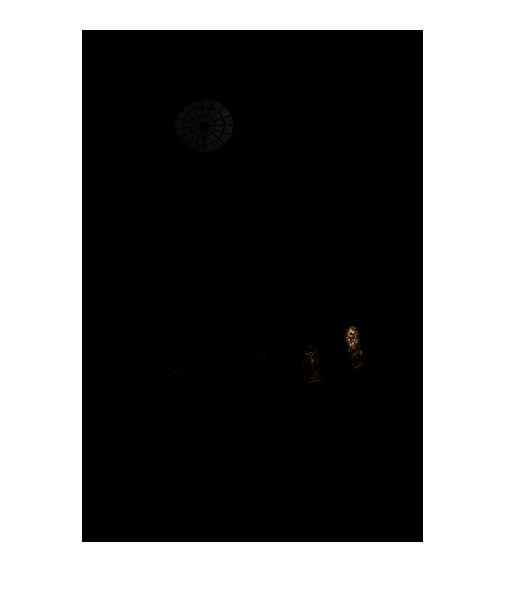
\includegraphics[width=\linewidth]{images/linearhdr1}
  	\caption{linear}\label{fig:logtonemap}
  	\endminipage\hfill
  	\minipage{0.48\textwidth}
  	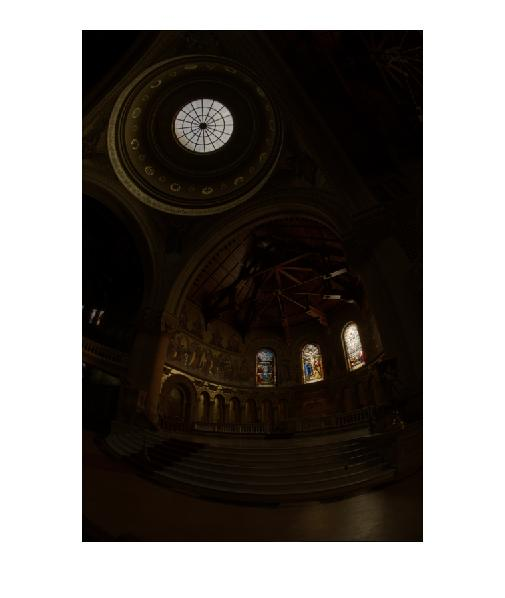
\includegraphics[width=\linewidth]{images/loghdr1}
  	\caption{logarithmic}\label{fig:lineartonemap}
  	\endminipage\hfill
  	% 	\centerline{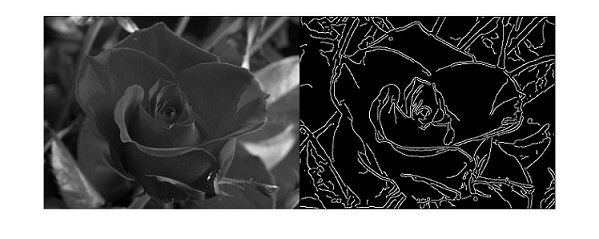
\includegraphics{images/cannyexample2}}
   \end{figure}
      
  \begin{figure}[!htb]
    \minipage{1\textwidth}
      	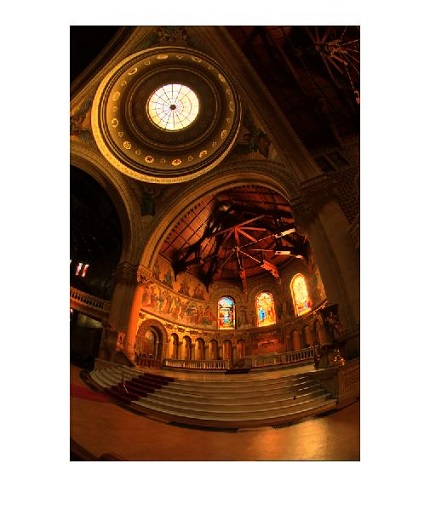
\includegraphics[width=\linewidth]{images/reinhardhdr1}
      	\caption{rainhard}\label{fig:logtonemap}
    \endminipage\hfill
      	% 	\centerline{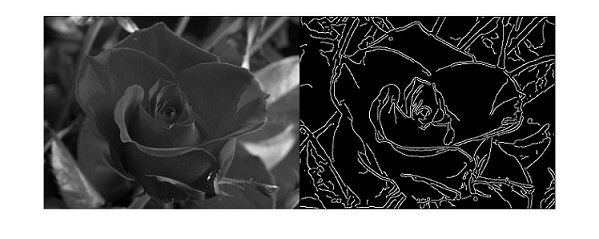
\includegraphics{images/cannyexample2}}
   \end{figure}
      
        
    \begin{figure}[!htb]
     \minipage{1\textwidth}
        	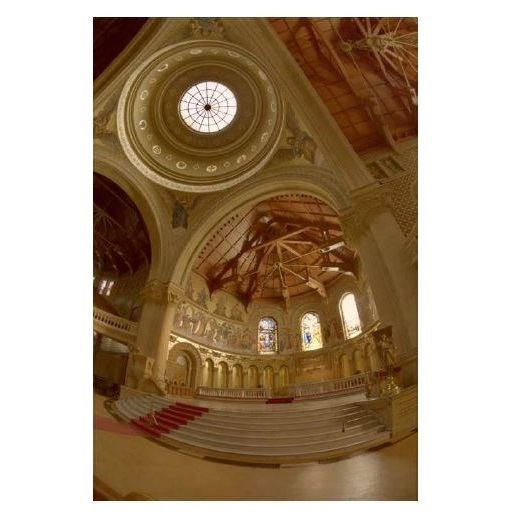
\includegraphics[width=\linewidth]{images/retinex3}
        	\caption{retinex}\label{fig:logtonemap}
      \endminipage\hfill
        	% 	\centerline{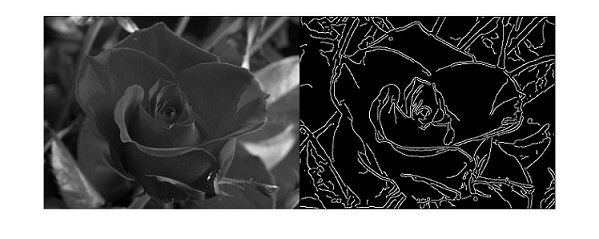
\includegraphics{images/cannyexample2}}
    \end{figure}
        
        
      \begin{figure}[!htb]
      	\minipage{0.48\textwidth}
      	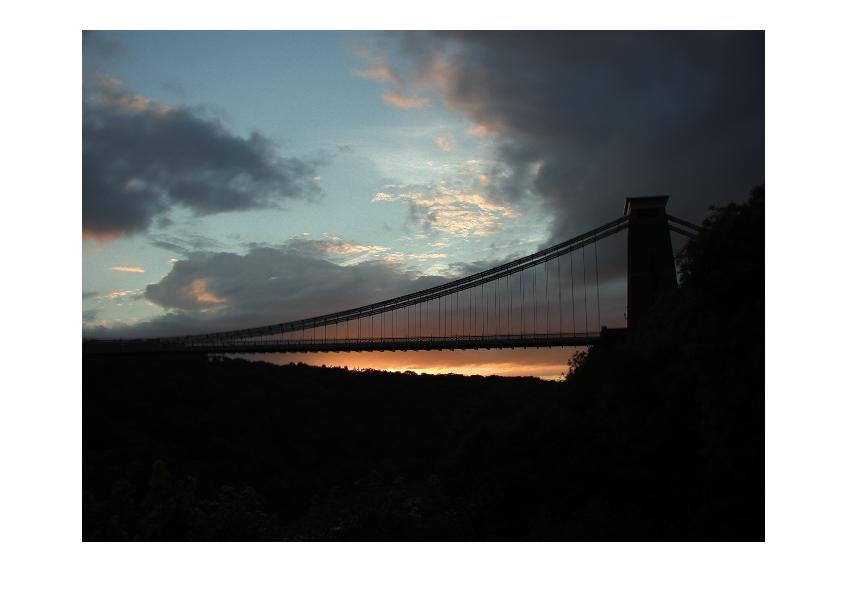
\includegraphics[width=\linewidth]{images/linearhdr3}
      	\caption{linear}\label{fig:logtonemap}
      	\endminipage\hfill
      	\minipage{0.48\textwidth}
      	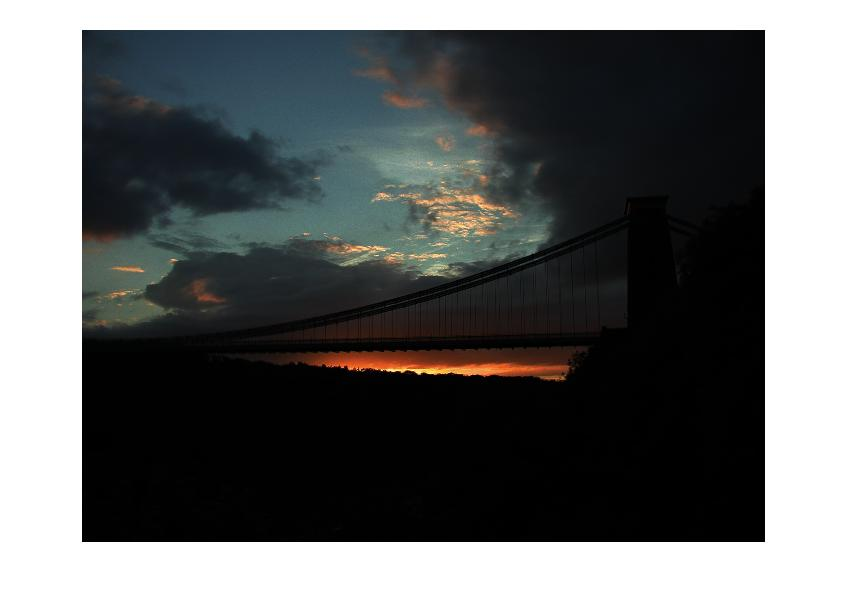
\includegraphics[width=\linewidth]{images/loghdr3}
      	\caption{logarithmic}\label{fig:lineartonemap}
      	\endminipage\hfill
      	% 	\centerline{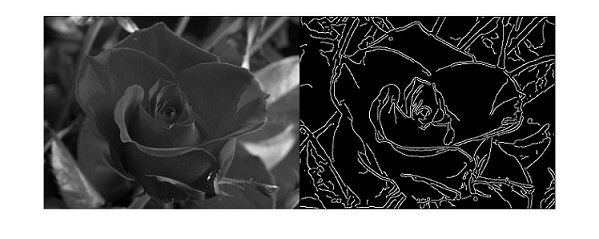
\includegraphics{images/cannyexample2}}
      \end{figure}
      
      \begin{figure}[!htb]
      	\minipage{1\textwidth}
      	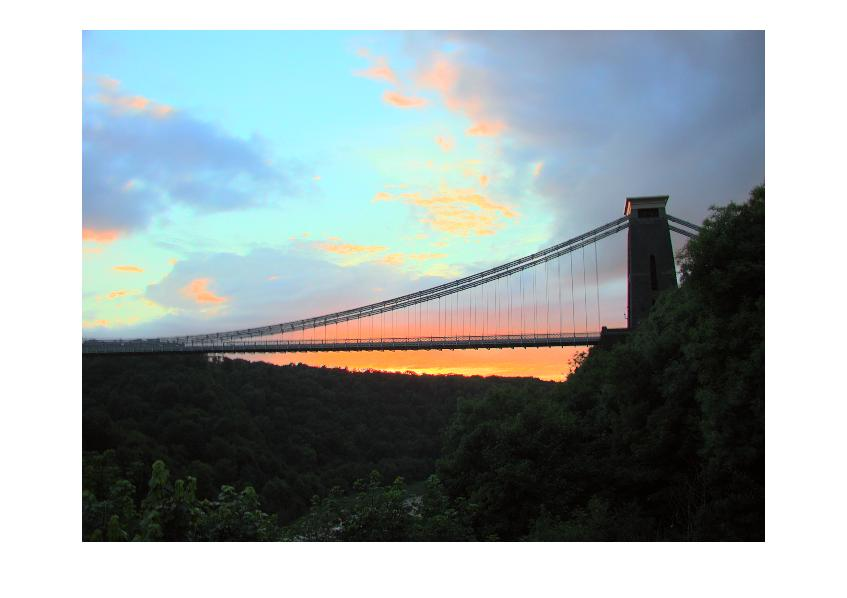
\includegraphics[width=\linewidth]{images/rainhardhdr3}
      	\caption{rainhard }\label{fig:logtonemap}
      	\endminipage\hfill
      	% 	\centerline{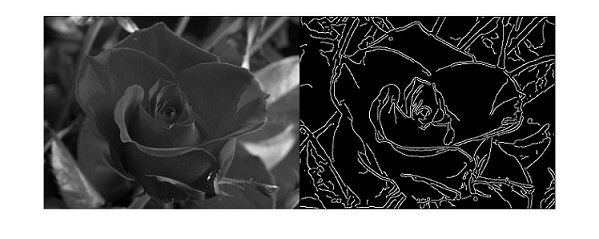
\includegraphics{images/cannyexample2}}
      \end{figure}
      
      
      \begin{figure}[!htb]
      	\minipage{1\textwidth}
      	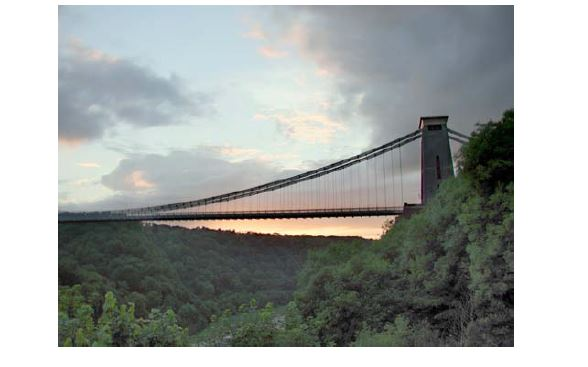
\includegraphics[width=\linewidth]{images/retinex1}
      	\caption{retinex}\label{fig:logtonemap}
      	\endminipage\hfill
      	% 	\centerline{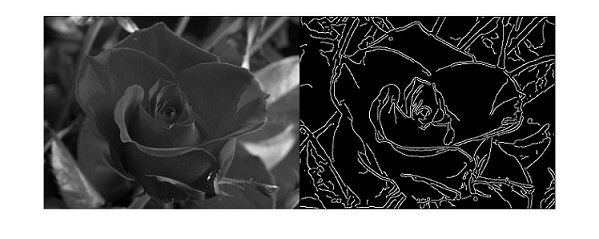
\includegraphics{images/cannyexample2}}
      \end{figure}
         